\documentclass[12pt,a4paper]{article}

\usepackage{geometry}
\geometry{top=2.3cm,bottom=2.4cm,left=2.1cm,right=2.1cm}

\usepackage[most]{tcolorbox}
\usepackage{xcolor}
\usepackage{tikz}
\usetikzlibrary{positioning,arrows.meta,calc}
\usepackage{fontawesome5}
\usepackage{setspace}
\usepackage{enumitem}
\usepackage{hyperref}
\usepackage{graphicx}
\usepackage{float}
\usepackage{listings}
\usepackage{fancyhdr}
\usepackage{titlesec}
\usepackage{array}
\usepackage{tabularx}
\usepackage{caption}
\usepackage{booktabs}
\usepackage{colortbl}
\usepackage{xepersian}

\IfFontExistsTF{B Nazanin}{\settextfont{B Nazanin}}{\IfFontExistsTF{Vazirmatn}{\settextfont{Vazirmatn}}{\settextfont{Amiri}}}
\IfFontExistsTF{Liberation Serif}{\setlatintextfont{Liberation Serif}}{\setlatintextfont{Times New Roman}}
\IfFontExistsTF{JetBrainsMono Nerd Font}{\setmonofont{JetBrainsMono Nerd Font}}{\setmonofont{DejaVu Sans Mono}}
\setstretch{1.35}

\definecolor{ink}{HTML}{20242A}
\definecolor{paper}{HTML}{FBFCFE}
\definecolor{midnight}{HTML}{263159}
\definecolor{navy}{HTML}{1E3A5F}
\definecolor{teal}{HTML}{0F766E}
\definecolor{green}{HTML}{10B981}
\definecolor{blue}{HTML}{3B82F6}
\definecolor{sky}{HTML}{EAF3FF}
\definecolor{mint}{HTML}{ECFDF3}
\definecolor{amber}{HTML}{F59E0B}
\definecolor{gold}{HTML}{E9B949}
\definecolor{softgold}{HTML}{FFF7D6}
\definecolor{rose}{HTML}{F43F5E}
\definecolor{lavender}{HTML}{F3E8FF}
\definecolor{violet}{HTML}{7C3AED}
\definecolor{softgray}{HTML}{F5F7FB}
\definecolor{linegray}{HTML}{D8DEE9}
\definecolor{tablehead}{HTML}{0F766E}
\definecolor{tablerow}{HTML}{F8FBFD}
\definecolor{tableline}{HTML}{C9D6E2}

\hypersetup{
colorlinks=true,
linkcolor=navy,
urlcolor=teal,
citecolor=teal
}

\pagecolor{paper}
\color{ink}
\setlength{\parindent}{0pt}
\setlength{\parskip}{0.55em}
\setlength{\arrayrulewidth}{0.45pt}
\setlength{\emergencystretch}{3em}

\captionsetup[table]{
labelfont={bf,color=teal},
textfont={color=ink},
skip=6pt
}

\newcommand{\tableheader}[1]{\bfseries #1}
\newcommand{\softmidrule}{\hline}

\newenvironment{tablecard}{%
\begin{tcolorbox}[
enhanced,
colback=white,
colframe=teal,
boxrule=0.8pt,
arc=4pt,
right=8pt,
left=8pt,
top=7pt,
bottom=7pt,
before skip=0.25em,
after skip=0.2em
]%
}{%
\end{tcolorbox}%
}

\setlist[itemize]{
label=\textcolor{teal}{\scriptsize\faCircle},
itemsep=0.25em,
topsep=0.3em,
rightmargin=1.4em
}

\setlist[enumerate]{
itemsep=0.25em,
topsep=0.3em,
rightmargin=1.4em
}

\lstdefinestyle{codestyle}{
basicstyle=\ttfamily\footnotesize,
breaklines=true,
frame=single,
backgroundcolor=\color{softgray},
rulecolor=\color{blue},
numbers=none,
xleftmargin=0pt,
xrightmargin=0pt,
aboveskip=0.6em,
belowskip=0.6em
}
\lstset{style=codestyle}

\newtcolorbox{tocbox}{
enhanced,
breakable,
colback=white,
colframe=teal,
boxrule=0.9pt,
arc=5pt,
right=12pt,
left=12pt,
top=10pt,
bottom=10pt,
title={\textcolor{white}{\faListUl\hspace{0.45em} فهرست مطالب}},
colbacktitle=teal,
coltitle=white,
fonttitle=\bfseries,
attach boxed title to top right={yshift=-2mm,xshift=-2mm},
boxed title style={arc=4pt,boxrule=0pt}
}

\newtcolorbox{infobox}[1]{
enhanced,
breakable,
colback=sky,
colframe=blue,
boxrule=0.8pt,
arc=5pt,
right=10pt,
left=10pt,
top=8pt,
bottom=8pt,
title={\textcolor{white}{\faInfoCircle\hspace{0.45em} #1}},
colbacktitle=blue,
coltitle=white,
fonttitle=\bfseries
}

\newtcolorbox{requirementbox}[1]{
enhanced,
breakable,
colback=mint,
colframe=green,
boxrule=0.8pt,
arc=5pt,
right=10pt,
left=10pt,
top=8pt,
bottom=8pt,
title={\textcolor{white}{\faCheckCircle\hspace{0.45em} #1}},
colbacktitle=green,
coltitle=white,
fonttitle=\bfseries
}

\newtcolorbox{warningbox}[1]{
enhanced,
breakable,
colback=softgold,
colframe=amber,
boxrule=0.8pt,
arc=5pt,
right=10pt,
left=10pt,
top=8pt,
bottom=8pt,
title={\textcolor{white}{\faExclamationTriangle\hspace{0.45em} #1}},
colbacktitle=amber,
coltitle=white,
fonttitle=\bfseries
}

\newtcolorbox{scorebox}[1]{
enhanced,
breakable,
colback=lavender,
colframe=violet,
boxrule=0.8pt,
arc=5pt,
right=10pt,
left=10pt,
top=8pt,
bottom=8pt,
title={\textcolor{white}{\faStar\hspace{0.45em} #1}},
colbacktitle=violet,
coltitle=white,
fonttitle=\bfseries
}

\newtcolorbox{questionbox}[1]{
enhanced,
breakable,
colback=white,
colframe=navy,
boxrule=0.8pt,
arc=5pt,
right=10pt,
left=10pt,
top=8pt,
bottom=8pt,
title={\textcolor{white}{\faQuestionCircle\hspace{0.45em} #1}},
colbacktitle=navy,
coltitle=white,
fonttitle=\bfseries
}

\newtcolorbox{reasonbox}[1]{
enhanced,
breakable,
colback=white,
colframe=teal,
boxrule=0.7pt,
arc=5pt,
right=10pt,
left=10pt,
top=8pt,
bottom=8pt,
title={\textcolor{white}{\faBalanceScale\hspace{0.45em} #1}},
colbacktitle=teal,
coltitle=white,
fonttitle=\bfseries
}

\titleformat{\section}
{\normalfont\Large\bfseries\color{midnight}}
{}
{0pt}
{\textcolor{gold}{\faBookOpen}\hspace{0.55em}}
[\vspace{0.25em}{\color{gold}\titlerule[0.9pt]}]

\titleformat{\subsection}
{\normalfont\large\bfseries\color{teal}}
{}
{0pt}
{\faBookmark\hspace{0.45em}}

\titleformat{\subsubsection}
{\normalfont\normalsize\bfseries\color{navy}}
{}
{0pt}
{\faAngleLeft\hspace{0.4em}}

\titlespacing*{\section}{0pt}{1.2em}{0.35em}
\titlespacing*{\subsection}{0pt}{0.9em}{0.2em}
\titlespacing*{\subsubsection}{0pt}{0.65em}{0.15em}

\pagestyle{plain}

\newcommand{\safelogo}[2]{%
\IfFileExists{#1}{\includegraphics[width=#2]{#1}}{\fbox{\parbox[c][1.8cm][c]{2.0cm}{\centering لوگو}}}%
}

\newcommand{\evidenceimage}[2]{%
\begin{minipage}{0.48\textwidth}
\centering
\includegraphics[width=\linewidth,height=6.2cm,keepaspectratio]{#1}
\captionof{figure}{#2}
\end{minipage}%
}

\newcommand{\makecover}{
\begin{titlepage}
\thispagestyle{empty}
\begin{tikzpicture}[remember picture,overlay]
\fill[midnight] (current page.south west) rectangle (current page.north east);
\fill[teal] (current page.north west) -- ++(0,-8.3) .. controls +(4.8,-1.1) and +(-4.8,1.3) .. ([yshift=-5.5cm]current page.north east) -- (current page.north east) -- cycle;
\fill[blue] ([xshift=1.0cm,yshift=1.0cm]current page.south west) circle (3.3cm);
\fill[gold] ([xshift=-2.25cm,yshift=-2.2cm]current page.north east) circle (3.25cm);
\fill[softgold] ([xshift=-2.25cm,yshift=-2.2cm]current page.north east) circle (2.25cm);
\draw[gold,line width=1.1pt] ([xshift=1.55cm,yshift=-10.7cm]current page.north west) -- ([xshift=-1.55cm,yshift=-10.7cm]current page.north east);
\draw[teal,line width=4pt] ([xshift=1.55cm,yshift=-11.2cm]current page.north west) -- ([xshift=1.55cm,yshift=2.0cm]current page.south west);
\draw[gold,line width=1.2pt] ([xshift=-1.55cm,yshift=-11.2cm]current page.north east) -- ([xshift=-1.55cm,yshift=2.0cm]current page.south east);
\end{tikzpicture}

\vspace*{1.15cm}
\begin{center}
\noindent
\begin{minipage}{0.18\textwidth}
\centering
\safelogo{ce.png}{2.05cm}
\end{minipage}
\begin{minipage}{0.56\textwidth}
\centering
\vspace{0.15cm}
{\Large\textcolor{softgold}{دانشگاه صنعتی امیرکبیر}}\\[0.15cm]
{\large\textcolor{white}{دانشکده مهندسی کامپیوتر}}
\end{minipage}
\begin{minipage}{0.18\textwidth}
\centering
\safelogo{aut.png}{2.15cm}
\end{minipage}\\[0.75cm]

{\Huge\bfseries\textcolor{gold}{فاز اول پروژه پایانی}}\\[0.45cm]
{\LARGE\textcolor{white}{تحلیل لاگ جام جهانی با Nginx و MapReduce}}\\[0.65cm]
{\textcolor{white}{\rule{0.72\textwidth}{0.8pt}}}\\[0.8cm]

\begin{tcolorbox}[
enhanced,
width=0.80\textwidth,
colback=white,
colframe=gold,
boxrule=1pt,
arc=5pt,
right=18pt,
left=18pt,
top=14pt,
bottom=14pt
]
\centering
{\Large\bfseries\textcolor{midnight}{مبانی رایانش ابری}}\\[0.35cm]
{\large\textcolor{teal}{نیمسال دوم ۱۴۰۴--۱۴۰۵}}\\[0.35cm]
{\large\bfseries\textcolor{midnight}{گزارش طراحی، پیاده‌سازی و آزمون}}
\end{tcolorbox}

\vspace{0.55cm}

\begin{tcolorbox}[
enhanced,
width=0.80\textwidth,
colback=softgray,
colframe=teal,
boxrule=0.9pt,
arc=5pt,
right=18pt,
left=18pt,
top=14pt,
bottom=14pt
]
\centering
{\large\bfseries\textcolor{midnight}{مشخصات گروه}}\\[0.25cm]
{\large\bfseries سید حسام الدین حسینیان}\quad{\large ۴۰۲۳۱۹۰۱}\\[0.18cm]
{\large\bfseries فروزان قویدل}\quad{\large ۴۰۲۳۱۰۶۴}\\[0.35cm]
{\large استاد درس: دکتر جوادی}\\
{\large تدریسیاران: مهرداد شیخ‌عباسی و محمدهادی ستاک}\\[0.5cm]

\end{tcolorbox}

\vfill
{\large\textcolor{softgold}{بهار ۱۴۰۵}}
\end{center}
\end{titlepage}
}

\begin{document}
\makecover
\setcounter{page}{1}

\begin{tocbox}
\small
\setcounter{tocdepth}{1}
\tableofcontents
\end{tocbox}

\clearpage
\section{صورت مسئله و محدوده کار}

هدف این فاز، ساخت یک مسیر کامل از تولید درخواست تا تحلیل نهایی لاگ بود. در این مسیر، سه سرویس اطلاعات بازی، تیم و ورزشگاه پشت یک درگاه Nginx قرار گرفتند. ترافیک آزمایشی فقط به Nginx ارسال شد، هر درخواست در دو سطح gateway و backend لاگ شد و در پایان، پنج مرحله پردازش دسته‌ای با Hadoop Streaming اجرا شد.

فایل دستورکار ۲۵ صفحه‌ای ابتدا به‌طور کامل بررسی شد. سپس موارد تحویلی به یک فهرست اجرایی تبدیل شد تا پیاده‌سازی به ترتیب انجام شود و هیچ خروجی اجباری جا نماند. بخش‌های اصلی کار عبارت بودند از:

\begin{itemize}
  \item تکمیل لاگ ساخت‌یافته در هر سه سرویس پایه؛
  \item نوشتن Dockerfile مستقل و فایل Compose برای سرویس‌ها؛
  \item تنظیم Nginx به عنوان تنها ورودی عمومی سامانه؛
  \item نوشتن traffic generator برای سناریوهای عادی، نامعتبر، کند، پرترافیک و خطای سرور؛
  \item تولید اجرای نهایی با حداقل ۱۰۰هزار درخواست؛
  \item پیاده‌سازی Jobهای 1 تا 5 با mapper و reducer پایتون؛
  \item اجرای واقعی Jobها با Hadoop Streaming و ذخیره همه خروجی‌های میانی و نهایی؛
  \item کنترل مصرف پردازنده و حافظه در تمام مراحل.
\end{itemize}

\begin{requirementbox}{نتیجه کلی}
اجرای نهایی شامل دقیقاً ۱۰۰٬۰۰۰ درخواست بود. فایل Nginx دقیقاً ۱۰۰٬۰۰۰ رکورد و مجموع سه فایل سرویس نیز ۱۰۰٬۰۰۰ رکورد داشت. پنج Job روی HDFS اجرا شدند و validator، سیزده خروجی اجباری را بدون خطا تأیید کرد.
\end{requirementbox}

\section{بررسی کد اولیه و برنامه اجرا}

در نسخه اولیه فقط فایل \lr{main.py} سه سرویس و Compose نمونه Hadoop وجود داشت. تابع \lr{write\_service\_log} در هر سه سرویس خالی بود و Dockerfile، پیکربندی Nginx، مولد ترافیک و کد MapReduce وجود نداشت. قالب گزارش نیز فقط شامل ظاهر و صفحه عنوان بود و بدنه‌ای نداشت.

برای کنترل ریسک، اجرا به سه سطح تقسیم شد:

\begin{enumerate}
  \item بررسی نحوی و تست مستقیم توابع بدون بالا آوردن سرویس‌های سنگین؛
  \item اجرای Debug با ۱۰۰۰ درخواست و تست محلی همان mapper/reducerها؛
  \item اجرای نهایی ۱۰۰هزار درخواست و سپس اجرای Hadoop، به‌صورت جدا از stack سرویس‌ها.
\end{enumerate}

در ابتدای کار سیستم ۷٫۴ گیگابایت RAM و ۱۶ پردازنده منطقی داشت، اما فقط حدود ۲٫۹ گیگابایت RAM در دسترس بود. به همین دلیل اجرای API و Hadoop هم‌زمان انجام نشد و برای تمام کانتینرها سقف منبع تعیین شد.

\section{معماری نهایی سامانه}

\begin{figure}[H]
\centering
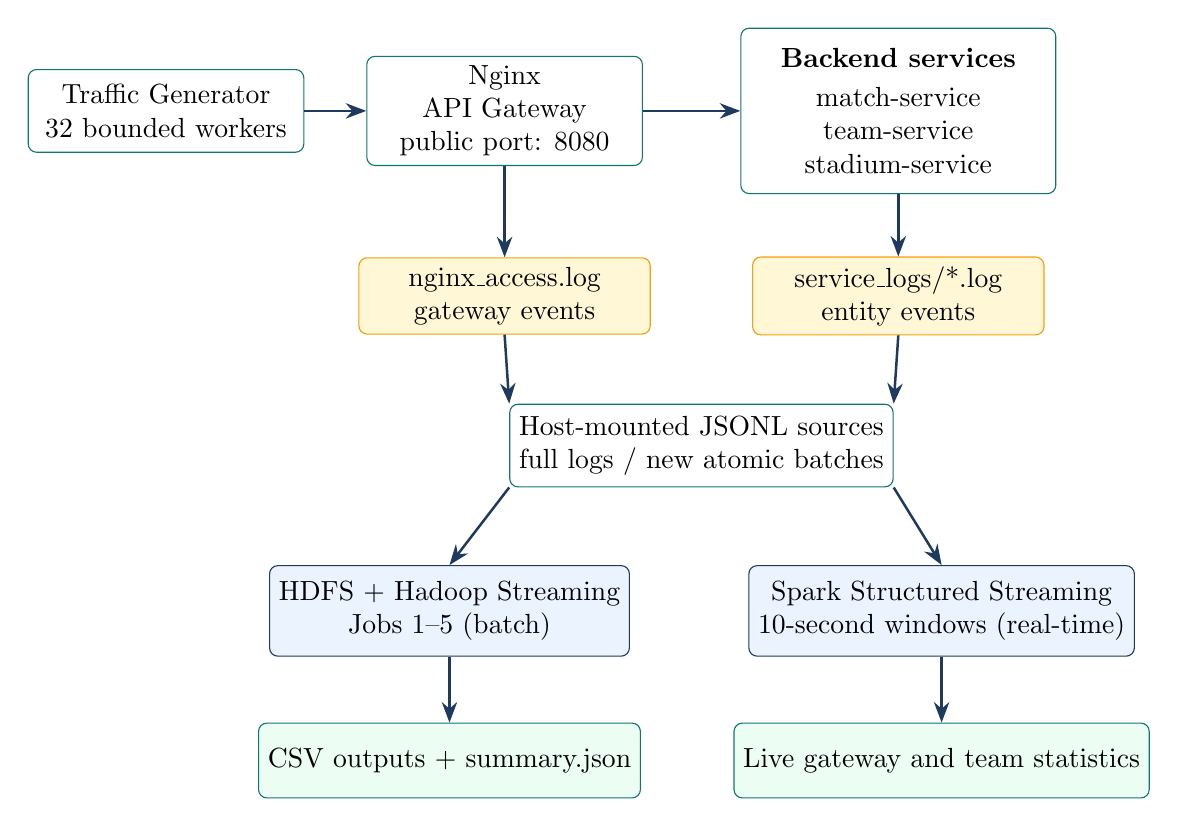
\begin{tikzpicture}[
box/.style={draw=teal,fill=white,rounded corners=3pt,minimum width=3.5cm,minimum height=1.05cm,align=center},
service/.style={box,minimum width=4.0cm,minimum height=2.1cm},
store/.style={draw=amber,fill=softgold,rounded corners=3pt,minimum width=3.7cm,minimum height=0.95cm,align=center},
stage/.style={draw=navy,fill=sky,rounded corners=3pt,minimum width=4.2cm,minimum height=1.15cm,align=center},
result/.style={draw=teal,fill=mint,rounded corners=3pt,minimum width=4.2cm,minimum height=0.95cm,align=center},
arr/.style={-{Stealth[length=2.6mm]},line width=0.9pt,color=navy}
]
\node[box] (gen) at (-5.6,2.6) {Traffic Generator\\\lr{32 bounded workers}};
\node[box] (nginx) at (-1.3,2.6) {Nginx\\API Gateway\\\lr{public port: 8080}};
\node[service] (services) at (3.7,2.6) {\textbf{Backend services}\\[2pt]
  \lr{match-service}\\\lr{team-service}\\\lr{stadium-service}};

\node[store] (nglog) at (-1.3,0.25) {\lr{nginx\_access.log}\\gateway events};
\node[store] (svclog) at (3.7,0.25) {\lr{service\_logs/*.log}\\entity events};
\node[box,minimum width=4.8cm] (source) at (1.2,-1.65)
  {Host-mounted JSONL sources\\full logs / new atomic batches};

\node[stage] (hadoop) at (-2.0,-3.75)
  {HDFS + Hadoop Streaming\\Jobs 1--5 (batch)};
\node[stage] (spark) at (4.25,-3.75)
  {Spark Structured Streaming\\10-second windows (real-time)};
\node[result] (outputs) at (-2.0,-5.65)
  {CSV outputs + \lr{summary.json}};
\node[result] (live) at (4.25,-5.65)
  {Live gateway and team statistics};

\draw[arr] (gen) -- (nginx);
\draw[arr] (nginx) -- (services);
\draw[arr] (nginx) -- (nglog);
\draw[arr] (services) -- (svclog);
\draw[arr] (nglog.south) -- (source.north west);
\draw[arr] (svclog.south) -- (source.north east);
\draw[arr] (source.south west) -- (hadoop.north);
\draw[arr] (source.south east) -- (spark.north);
\draw[arr] (hadoop) -- (outputs);
\draw[arr] (spark) -- (live);
\end{tikzpicture}
\caption{معماری نهایی سامانه و مسیر جداگانه پردازش batch و real-time}
\end{figure}

هیچ پورت backend روی میزبان publish نشده است. بنابراین مولد ترافیک از بیرون شبکه Docker راهی برای دور زدن Nginx ندارد و تنها پورت عمومی، \lr{8080} است.

\section{پیاده‌سازی سرویس‌های Backend}

\subsection{تکمیل لاگ ساخت‌یافته}

در هر سه سرویس، یک رکورد JSON مستقل برای هر درخواست نوشته می‌شود. برای جلوگیری از مخلوط شدن خطوط در درخواست‌های هم‌زمان، نوشتن فایل با \lr{threading.Lock} محافظت شد. مسیر فایل نیز از متغیر محیطی خوانده می‌شود تا کد به مسیر مطلق سیستم شخصی وابسته نباشد.

\begin{table}[H]
\centering
{\bfseries\color{teal} فیلدهای ثبت‌شده در لاگ سرویس‌ها}\par\medskip
\begin{tablecard}
\begin{tabularx}{\textwidth}{>{\bfseries\color{teal}}l X}
\toprule
فیلد & کاربرد \\
\midrule
\lr{timestamp} & زمان UTC با قالب ISO-8601 \\
\lr{request\_id} & شناسه منتقل‌شده از Nginx برای تطبیق دو لاگ \\
\lr{client\_country} & کشور کاربر آزمایشی \\
\lr{scenario} & نوع سناریوی ترافیک؛ این فیلد افزون بر حداقل schema نگه داشته شد \\
\lr{service, endpoint} & نام سرویس و مسیر بدون query \\
\lr{entity\_type/value} & نوع و مقدار تیم، روز مسابقه، ورزشگاه یا شهر \\
\lr{status\_code} & کد واقعی پاسخ \\
\lr{processing\_time\_ms} & زمان پردازش داخل سرویس \\
\lr{event\_type} & نوع رخداد جست‌وجو \\
\bottomrule
\end{tabularx}
\end{tablecard}
\end{table}

رفتار endpointهای اولیه حفظ شد: ورودی معتبر پاسخ ۲۰۰، ورودی ناقص یا با قالب نامعتبر پاسخ ۴۰۰، موجودیت ناموجود پاسخ ۴۰۴ و سناریوی \lr{server\_error} پاسخ ۵۰۰ می‌دهد. سناریوی \lr{slow} نیز تأخیر کنترل‌شده ایجاد می‌کند.

\subsection{Dockerfile و محدودیت منابع}

برای هر سرویس Dockerfile مستقل بر پایه \lr{python:3.12-slim} نوشته شد. وابستگی‌ها به نسخه مشخص \lr{FastAPI 0.116.1} و \lr{Uvicorn 0.35.0} محدود شدند. هر سرویس فقط یک worker دارد و access log تکراری Uvicorn غیرفعال شده است.

\begin{table}[H]
\centering
{\bfseries\color{teal} محدودیت منابع stack سرویس‌ها}\par\medskip
\begin{tablecard}
\begin{tabular}{lccc}
\toprule
جزء & سقف RAM & سقف CPU & سقف process \\
\midrule
match-service & \lr{160 MB} & \lr{0.50} & ۱۲۸ \\
team-service & \lr{160 MB} & \lr{0.50} & ۱۲۸ \\
stadium-service & \lr{160 MB} & \lr{0.50} & ۱۲۸ \\
Nginx & \lr{64 MB} & \lr{0.25} & ۶۴ \\
\bottomrule
\end{tabular}
\end{tablecard}
\end{table}

\begin{figure}[H]
\centering
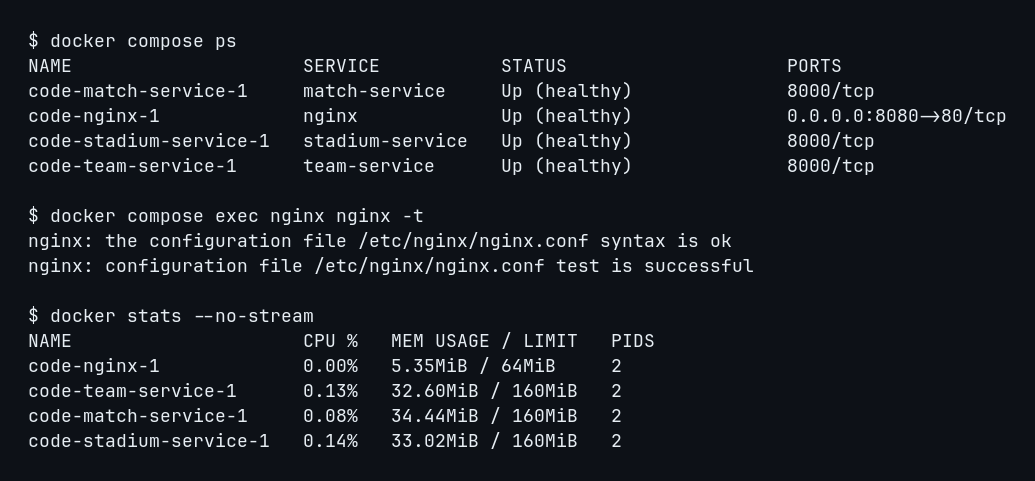
\includegraphics[width=0.96\textwidth]{evidence/01_services.png}
\caption{اجرای موفق کانتینرها، تست کانفیگ Nginx و مصرف پایه منابع}
\end{figure}

\section{تنظیم Nginx}

Nginx با یک worker و ۱۰۲۴ اتصال تنظیم شد. سه upstream جداگانه تعریف شدند و مسیرهای زیر به سرویس متناظر فرستاده می‌شوند:

\begin{itemize}
  \item \lr{/api/matches} به match-service؛
  \item \lr{/api/teams} به team-service؛
  \item \lr{/api/stadiums} به stadium-service.
\end{itemize}

سه header اصلی با \lr{proxy\_set\_header} منتقل می‌شوند. اگر \lr{X-Request-ID} فرستاده نشود، Nginx شناسه داخلی خود را جایگزین می‌کند؛ کشور پیش‌فرض \lr{unknown} و سناریوی پیش‌فرض \lr{normal} است. access log با \lr{escape=json} و به شکل JSON Lines در \lr{data/nginx/nginx\_access.log} نوشته می‌شود.

برای کاهش I/O، بافر ۶۴ کیلوبایتی و flush یک‌ثانیه‌ای برای access log در نظر گرفته شد. همین موضوع هنگام پاک‌سازی اجرای Debug مهم بود و در بخش خطاهای حین اجرا توضیح داده شده است.

\begin{figure}[H]
\centering
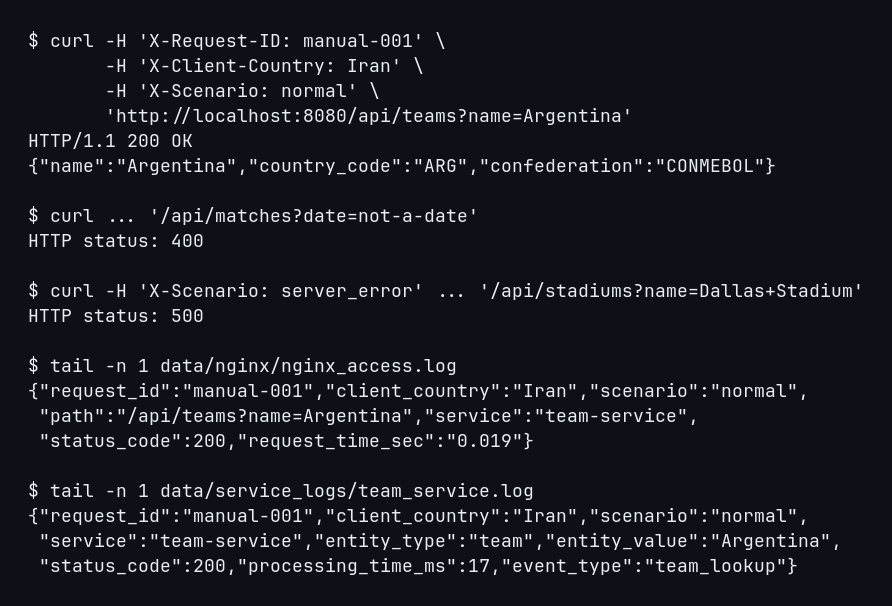
\includegraphics[width=0.94\textwidth]{evidence/02_gateway_test.png}
\caption{تست مسیر Nginx، پاسخ‌های ۲۰۰/۴۰۰/۵۰۰ و تطبیق دو سطح لاگ}
\end{figure}

\section{مولد ترافیک}

مولد ترافیک فقط از کتابخانه استاندارد پایتون استفاده می‌کند. برای جلوگیری از مصرف حافظه بالا، ۱۰۰هزار Future ساخته نمی‌شود؛ فقط تعداد ثابتی worker ایجاد می‌شود و هر worker یک دنباله از شماره درخواست‌ها را پردازش می‌کند. هر worker اتصال HTTP خود را reuse می‌کند و در خطای شبکه فقط یک بار اتصال را بازسازی می‌کند.

ترکیب هدف ترافیک به‌صورت وزنی تعریف شد تا تفاوت سرویس‌ها و موجودیت‌ها در خروجی دیده شود:

\begin{itemize}
  \item حدود ۵۰ درصد تیم، ۲۸ درصد مسابقه و ۲۲ درصد ورزشگاه؛
  \item سناریوهای \lr{normal}، \lr{popular}، \lr{invalid}، \lr{server\_error} و \lr{slow}؛
  \item هشت کشور با علاقه غالب متفاوت برای هر کشور؛
  \item توزیع نامتوازن به نفع آرژانتین، تاریخ ۲۵ ژوئن و ورزشگاه New York New Jersey؛
  \item شناسه یکتا با قالب \lr{req\_000001} تا \lr{req\_100000}.
\end{itemize}

ابتدا ۱۰۰۰ درخواست با ۸ worker اجرا شد. این تست در ۵٫۲۸ ثانیه تمام شد و شامل ۹۶۷ پاسخ 2xx، بیست پاسخ 4xx و سیزده پاسخ 5xx بود. سپس منطق پنج Job به‌صورت محلی روی همین لاگ تست شد. این تست محلی فقط برای debug بود و جای اجرای Hadoop را نگرفت.

\subsection{اجرای نهایی}

اجرای نهایی با ۳۲ اتصال محدود انجام شد. زمان کل ۱۱۹٫۷۷ ثانیه و نرخ میانگین ۸۳۴٫۹ درخواست در ثانیه بود.

\begin{figure}[H]
\centering
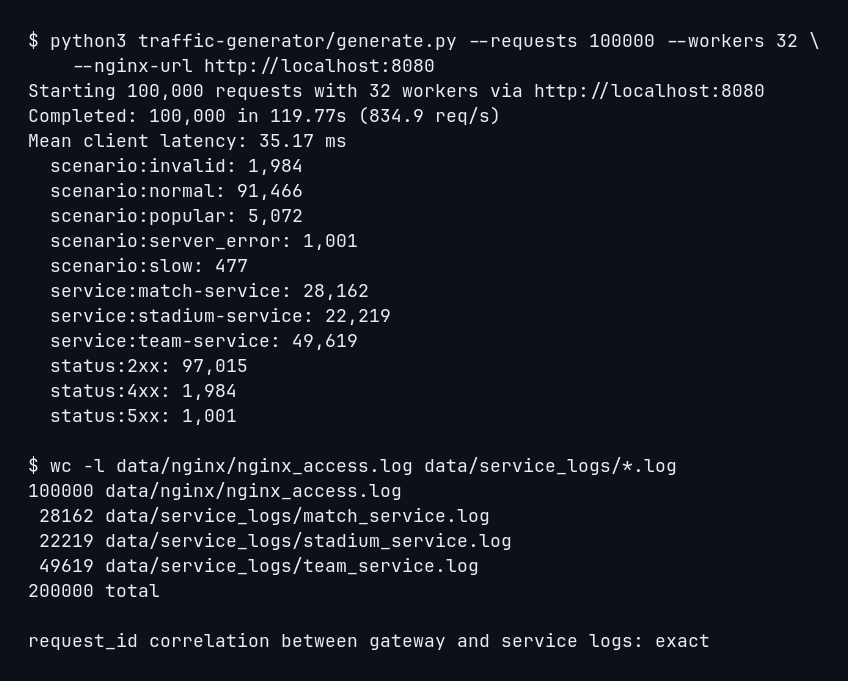
\includegraphics[width=0.94\textwidth]{evidence/03_final_traffic.png}
\caption{خروجی اجرای نهایی ۱۰۰هزار درخواست و شمارش فایل‌های لاگ}
\end{figure}

پس از پایان، تمام خطوط چهار فایل با parser استاندارد JSON بررسی شد. شناسه‌ها در هر فایل یکتا بودند و مجموعه شناسه‌های لاگ Nginx دقیقاً با اجتماع شناسه‌های سه لاگ سرویس برابر بود. حجم فایل Nginx حدود ۲۹ مگابایت و مجموع لاگ سرویس‌ها حدود ۲۸ مگابایت شد.

\section{خطاهای مشاهده‌شده و اصلاح آن‌ها}

در اجرای واقعی دو نکته مشخص شد که در تست کاغذی دیده نمی‌شد:

\subsection{مالکیت فایل‌های bind mount}

فایل‌های لاگ در بار اول با مالک root کانتینر ساخته شدند و کاربر میزبان اجازه truncate نداشت. اجرای نهایی فوراً متوقف شد، فایل‌های مشخص از داخل کانتینر truncate شدند و مالکیت پوشه‌های لاگ به کاربر میزبان برگردانده شد. هیچ فایل دیگری حذف نشد.

\subsection{بافر Nginx پس از توقف ترافیک}

چند درخواست در حال اجرا و داده موجود در بافر یک‌ثانیه‌ای، بعد از truncate اولیه وارد فایل شدند. برای اینکه شمار نهایی دقیقاً ۱۰۰هزار باشد، stack کامل stop شد، فایل‌ها پس از تخلیه بافر صفر شدند و سپس سرویس‌ها دوباره بالا آمدند. health check مسیر جداگانه‌ای دارد و در access log ثبت نمی‌شود؛ بنابراین اجرای نهایی از صفر واقعی شروع شد.

\subsection{توقف امن traffic generator}

در نسخه نخست، \lr{KeyboardInterrupt} می‌توانست process اصلی را متوقف کند ولی threadهای در حال کار برای چند لحظه ادامه دهند. یک \lr{Event} مشترک و shutdown کنترل‌شده اضافه شد تا هر worker پس از درخواست جاری خارج شود و process پس‌زمینه باقی نماند.

\subsection{نسخه پایتون image نمونه Hadoop}

image ارائه‌شده Python 3.5 نصب می‌کرد، در حالی که چند پیام قالب‌بندی mapperها در ابتدا f-string داشتند. قبل از اجرای Jobها این ناسازگاری پیدا شد، f-stringها به \lr{str.format} تبدیل شدند و همه mapper/reducerها داخل خود NameNode با Python 3.5 کامپایل شدند.

\subsection{محدودیت thread در اجرای Spark}

در دو اجرای نخست بخش امتیازی، آمار زنده درست در ترمینال دیده شد اما هنگام ذخیره جداگانه هر micro-batch، فراخوانی‌های متعدد فایل‌سیستم محلی تعداد thread/process را به سقف ۲۵۶ رساند. ابتدا JVM با \lr{ActiveProcessorCount=2} محدود شد؛ این کار اندازه poolهای داخلی را کم کرد، ولی نوشتن هم‌زمان خروجی و checkpoint هنوز سربار غیرضروری داشت. چون طبق صورت پروژه نمایش زنده در ترمینال یکی از خروجی‌های قابل قبول است، نوشتن تکراری JSON حذف و checkpoint حفظ شد. اجرای سوم با همان سقف ۲۵۶، حداکثر ۶۲ PID و کد خروج صفر تمام شد. بررسی وضعیت هر دو query نیز به حلقه اجرا اضافه شد تا خطای یکی از جریان‌ها پنهان نماند.



\section{راه‌اندازی Hadoop و HDFS}

Compose نمونه حفظ و با ساختار پروژه هماهنگ شد. کل پروژه روی \lr{/project} mount می‌شود. نصب Python فقط در NameNode انجام می‌شود، چون DataNode mapper یا reducer اجرا نمی‌کند. محدودیت NameNode برابر ۱۲۰۰ مگابایت و یک CPU، و محدودیت DataNode برابر ۷۰۰ مگابایت و نیم CPU تعیین شد.

پس از healthy شدن دو کانتینر، \lr{hdfs dfsadmin -report} وجود یک DataNode زنده را تأیید کرد. فایل‌های ورودی ابتدا از volume محلی دیده شدند و سپس با \lr{hdfs dfs -put} واقعاً روی HDFS قرار گرفتند.

\begin{figure}[H]
\centering
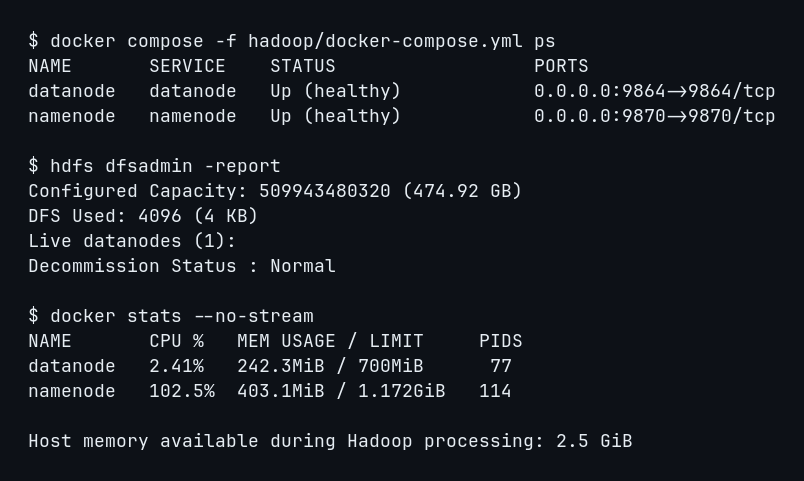
\includegraphics[width=0.92\textwidth]{evidence/04_hadoop_cluster.png}
\caption{وضعیت کلاستر، DataNode زنده و مصرف منابع هنگام Hadoop Streaming}
\end{figure}

\section{پیاده‌سازی پنج Job با Hadoop Streaming}

تمام Jobها با یک reducer اجرا شدند تا مصرف حافظه پایین بماند و فایل خروجی نهایی قطعی باشد. برای taskهای map و reduce سقف ۲۵۶ مگابایت و heap برابر ۱۹۲ مگابایت تعیین شد. اسکریپت \lr{scripts/run\_mapreduce.sh} پوشه‌های HDFS را می‌سازد، ورودی‌ها را upload می‌کند، خروجی قبلی هر Job را حذف می‌کند، Jobها را به ترتیب اجرا می‌کند، فایل‌های HDFS را به \lr{outputs/} برمی‌گرداند و در پایان schemaها را اعتبارسنجی می‌کند.

\subsection{Job 1: Parsing and Cleaning}

ورودی Job 1 شامل ۱۰۰هزار خط Nginx و ۱۰۰هزار خط سرویس بود. mapper نوع رکورد را از schema تشخیص می‌دهد، وجود تمام فیلدهای اجباری و عددی بودن status/time را بررسی می‌کند و زمان Nginx را از ثانیه به میلی‌ثانیه تبدیل می‌کند. رکوردها با tagهای \lr{nginx}، \lr{service} و \lr{invalid} به reducer می‌روند. reducer داده معتبر را بدون بارگذاری کامل در حافظه عبور می‌دهد.

خروجی واقعی Hadoop شامل ۲۰۰هزار رکورد بود. پس از جداسازی tagها، دو CSV صد‌هزارردیفی ساخته شد و \lr{invalid\_logs.csv} فقط header داشت؛ خالی بودن بخش داده invalid طبیعی است، زیرا تولیدکننده لاگ schema ثابت دارد.

\subsection{Job 2: General Nginx Aggregation}

mapper برای هر رکورد سه کلید service، endpoint و scenario تولید می‌کند. مقدار هر کلید شامل شمار کل، موفق، 4xx، 5xx و زمان پاسخ است. reducer مجموع، نرخ خطا و میانگین زمان را حساب می‌کند. ۱۰۰هزار ورودی به ۳۰۰هزار زوج میانی و در نهایت ۱۱ ردیف آماری تبدیل شد.

\subsection{Job 3: Country--Entity Request Count}

این Job فقط از \lr{cleaned\_service\_logs.csv} استفاده می‌کند. کلید mapper شامل کشور، سرویس، نوع موجودیت و مقدار آن است و reducer تعداد را جمع می‌کند. موجودیت خالی وارد تحلیل محبوبیت نمی‌شود. خروجی نهایی شامل ۲۶۴ ترکیب یکتا بود و به سه فایل تیم، تاریخ و ورزشگاه/شهر تقسیم شد.

\subsection{Job 4: Popular Entity by Country}

ورودی مستقیم این مرحله خروجی HDFS مربوط به Job 3 است. mapper داده‌ها را بر اساس کشور گروه‌بندی می‌کند و reducer بیشترین count را انتخاب می‌کند. در تساوی، ترتیب الفبایی برای نتیجه قطعی استفاده می‌شود. سه فایل محبوب‌ترین تیم، روز مسابقه و ورزشگاه هر کشور تولید شد.

\subsection{Job 5: Final Report Generation}

این مرحله خروجی‌های Jobهای 2، 3 و 4 و فایل metadata پیش‌بینی مسابقات را می‌خواند. reducer تنها یک شیء JSON می‌سازد. مجموع درخواست‌ها از آمار سرویس‌های Job 2، محبوب‌ترین موجودیت کلی از جمع Job 3 و محبوب‌ترین تیم هر کشور از Job 4 به دست می‌آید. اطلاعات فینال پیش‌بینی‌شده نیز از داده ثابت سناریوی سرویس مسابقه وارد metadata شده است.

\begin{figure}[H]
\centering
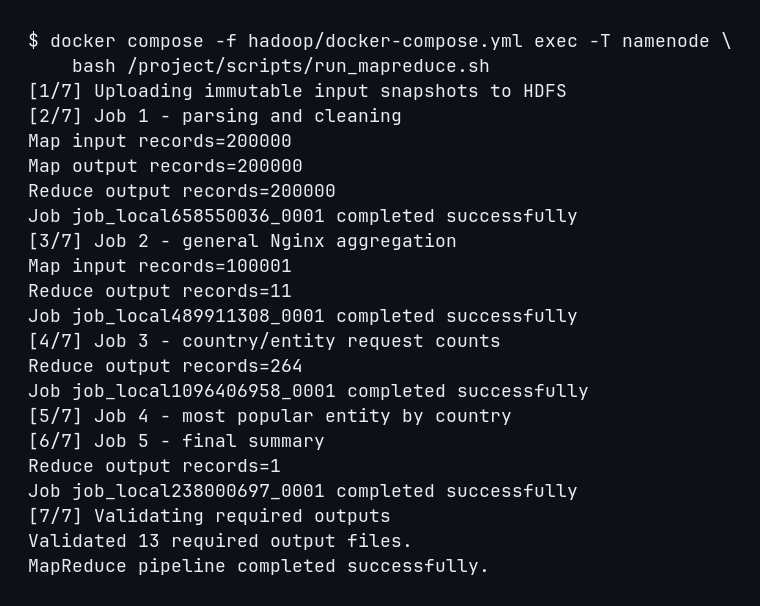
\includegraphics[width=0.94\textwidth]{evidence/05_mapreduce_run.png}
\caption{اجرای پشت‌سرهم Jobها و تأیید سیزده خروجی الزامی}
\end{figure}

\section{تحلیل خروجی‌ها}

\subsection{آمار سرویس‌ها}

\begin{table}[H]
\centering
{\bfseries\color{teal} خروجی \lr{outputs/job2/service\_stats.csv}}\par\medskip
\begin{tablecard}
\begin{tabular}{lrrrrr}
\toprule
سرویس & کل & موفق & 4xx & 5xx & میانگین زمان (ms) \\
\midrule
match-service & ۲۸٬۱۶۲ & ۲۷٬۲۹۲ & ۵۶۳ & ۳۰۷ & ۳۷٫۲۶۵ \\
stadium-service & ۲۲٬۲۱۹ & ۲۱٬۵۶۵ & ۴۵۱ & ۲۰۳ & ۳۶٫۵۶۴ \\
team-service & ۴۹٬۶۱۹ & ۴۸٬۱۵۸ & ۹۷۰ & ۴۹۱ & ۳۲٫۷۲۳ \\
\bottomrule
\end{tabular}
\end{tablecard}
\end{table}

team-service با ۴۹٬۶۱۹ درخواست پرترافیک‌ترین سرویس شد. نرخ خطای match-service برابر ۳٫۰۸۹۳ درصد و کمی بیشتر از دو سرویس دیگر بود؛ بنابراین در summary به عنوان سرویس با بیشترین نرخ خطا ثبت شد. میانگین زمان match-service نیز بیشترین مقدار بود و \lr{/api/matches} به عنوان کندترین endpoint انتخاب شد.

\subsection{اثر سناریوی کند}

سناریوی \lr{slow} شامل ۴۷۷ درخواست موفق و میانگین زمان ۸۰۱٫۲۲۶ میلی‌ثانیه بود. در مقابل، میانگین سناریوهای عادی و popular نزدیک ۳۱ میلی‌ثانیه ماند. این فاصله نشان می‌دهد داده برای تحلیل response time تنوع کافی دارد.

\subsection{محبوبیت موجودیت‌ها}

به دلیل توزیع هدفمند، تیم محبوب کلی Argentina، تاریخ پرتکرار \lr{2026-06-25} و ورزشگاه پرتکرار New York New Jersey Stadium شد. با این حال، علاقه تیمی هر کشور مستقل است: برای مثال Iran بیشترین درخواست را برای Iran و Germany بیشترین درخواست را برای Germany داشته است. این نتیجه نشان می‌دهد header کشور واقعاً تا لاگ سرویس منتقل و در Jobهای 3 و 4 استفاده شده است.

\begin{figure}[H]
\centering
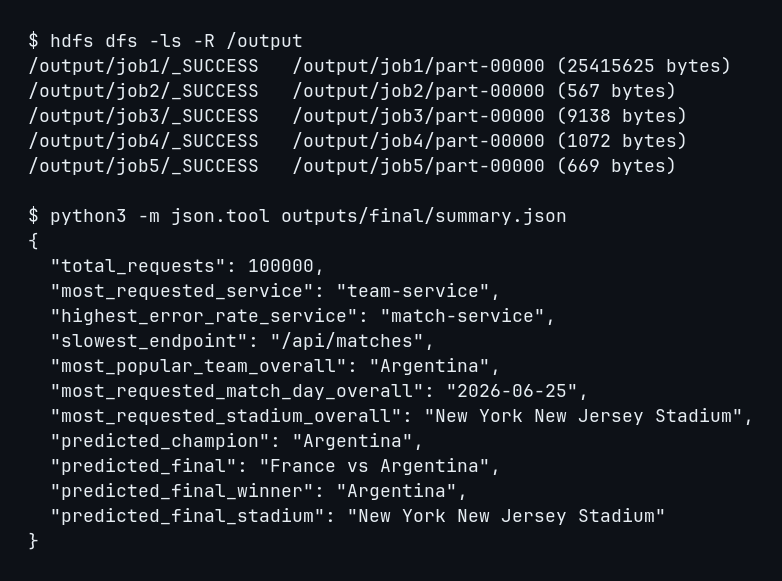
\includegraphics[width=0.92\textwidth]{evidence/06_final_output.png}
\caption{وجود خروجی همه Jobها روی HDFS و محتوای summary نهایی}
\end{figure}

\section{بخش امتیازی Spark Structured Streaming}

این بخش پس از پایان کامل Hadoop اجرا شد تا مصرف دو stack روی هم جمع نشود. image رسمی \lr{apache/spark:3.5.5} با \lr{local[2]} اجرا شد. سقف کانتینر ۱۶۰۰ مگابایت RAM و دو CPU، حافظه driver برابر ۷۶۸ مگابایت و تعداد shuffle partition برابر دو است. رابط وب Spark نیز غیرفعال شد.

برنامه دو \lr{readStream} مستقل با schema صریح دارد. جریان اول فایل‌های تازه Nginx را می‌خواند، \lr{request\_time\_sec} رشته‌ای را به \lr{double} و سپس میلی‌ثانیه تبدیل می‌کند و در پنجره‌های ده‌ثانیه‌ای، تعداد درخواست، تعداد خطا، نرخ خطا و میانگین زمان پاسخ را به تفکیک سرویس و endpoint می‌سازد. جریان دوم لاگ سرویس را می‌خواند و محبوب‌ترین تیم هر کشور را در همان پنجره زمانی محاسبه می‌کند. watermark سی‌ثانیه‌ای و دو مسیر checkpoint مستقل برای محدودکردن state و ادامه قابل اعتماد جریان در نظر گرفته شد.

اسکریپت \lr{export\_log\_batches.py} خطوط منبع را در فایل‌های ۲۰۰تایی می‌ریزد. هر batch ابتدا با پسوند موقت نوشته و سپس با rename اتمیک وارد پوشه stream می‌شود؛ در نتیجه Spark فایل نیمه‌نوشته را نمی‌خواند. در آزمون نهایی این بخش، پنج فایل Nginx و پنج فایل سرویس، هرکدام در مجموع ۱۰۰۰ رکورد، هنگام فعال بودن queryها وارد شدند. مقدارهای epoch صفر پس از رسیدن فایل‌های جدید ظاهر شدند و process با کد صفر خاتمه یافت.

\begin{figure}[H]
\centering
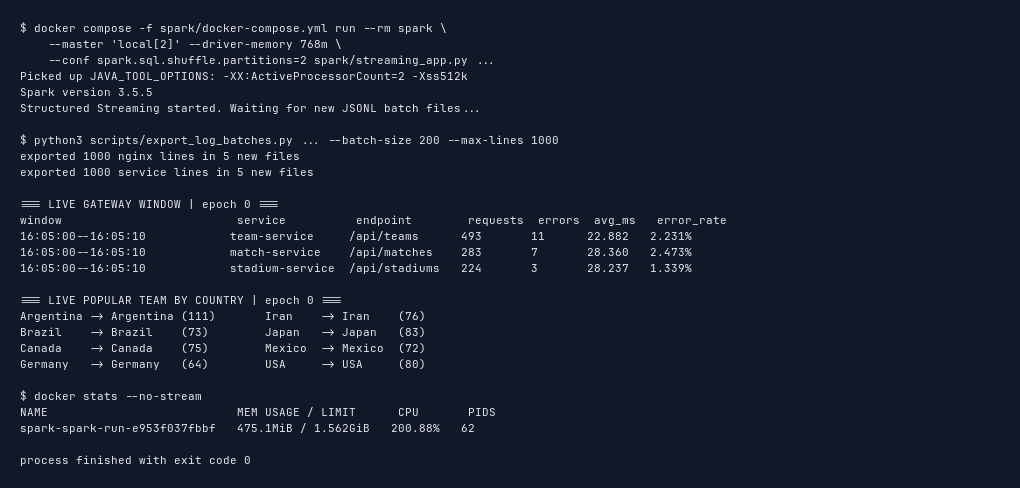
\includegraphics[width=0.96\textwidth]{evidence/07_spark_streaming.png}
\caption{خروجی زنده Spark پس از ورود batchهای جدید و مصرف منابع اجرای نهایی}
\end{figure}

\section{کنترل مصرف RAM و CPU}

کنترل منابع فقط در فایل Compose نبود و در زمان اجرا نیز اندازه‌گیری شد:

\begin{itemize}
  \item در حالت idle مجموع RAM چهار کانتینر API حدود ۱۰۶ مگابایت بود؛
  \item زیر بار ۳۲ اتصال، Nginx حدود ۶٫۳ مگابایت و سرویس‌ها حدود ۵۰، ۳۹ و ۳۷ مگابایت مصرف کردند؛
  \item traffic generator فقط ۳۲ worker ثابت داشت و فهرست ۱۰۰هزار Future در حافظه نساخت؛
  \item API و Hadoop هم‌زمان اجرا نشدند؛ فایل‌های لاگ روی میزبان باقی ماندند و بعد از stop سرویس‌ها Hadoop شروع شد؛
  \item در حین Job 1، NameNode همراه process پردازش حدود ۴۰۳ مگابایت و DataNode حدود ۲۴۲ مگابایت RAM داشت؛
  \item در همان لحظه حدود ۲٫۵ گیگابایت RAM سیستم available بود و هیچ کانتینری به سقف حافظه نرسید.
  \item Hadoop پیش از Spark خاموش شد؛ Spark در اجرای موفق حدود ۴۷۵ مگابایت RAM، دو هسته CPU و ۶۲ PID مصرف کرد.
\end{itemize}

\section{آزمون‌ها و معیار پذیرش}

\begin{table}[H]
\centering
{\bfseries\color{teal} جمع‌بندی آزمون‌های انجام‌شده}\par\medskip
\begin{tablecard}
\begin{tabularx}{\textwidth}{>{\bfseries}X l}
\toprule
آزمون & نتیجه \\
\midrule
کامپایل نحوی سه سرویس و همه mapper/reducerها & موفق \\
اعتبارسنجی \lr{docker compose config} & موفق \\
تست \lr{nginx -t} داخل image واقعی & موفق \\
health check چهار کانتینر API & healthy \\
پاسخ دستی ۲۰۰، ۴۰۰ و ۵۰۰ از مسیر Nginx & موفق \\
اجرای Debug با حداقل ۱۰۰۰ درخواست & ۱۰۰۰ درخواست \\
اجرای نهایی & دقیقاً ۱۰۰٬۰۰۰ درخواست \\
parse تمام خطوط JSON & بدون رکورد خراب \\
یکتایی و تطبیق request ID در دو سطح لاگ & تطبیق دقیق \\
DataNode زنده در \lr{dfsadmin -report} & یک DataNode \\
Jobهای 1 تا 5 روی Hadoop Streaming & همه موفق \\
اعتبارسنجی فایل‌های خروجی & ۱۳ فایل معتبر \\
Spark Structured Streaming با ورودی تدریجی & ۲۰۰۰ رکورد، کد خروج صفر \\
\bottomrule
\end{tabularx}
\end{tablecard}
\end{table}

\section{روش اجرای پروژه}

\subsection{سرویس‌ها و ترافیک}

\begin{latin}
\begin{lstlisting}[language=bash]
cd code_phase1/code
docker compose up --build -d
docker compose ps
docker compose exec nginx nginx -t

python3 traffic-generator/generate.py \
  --requests 1000 --workers 8 \
  --nginx-url http://localhost:8080

python3 traffic-generator/generate.py \
  --requests 100000 --workers 32 \
  --nginx-url http://localhost:8080
\end{lstlisting}
\end{latin}

برای شروع یک اجرای تمیز، ابتدا stack متوقف می‌شود و سپس چهار فایل لاگ مشخص truncate می‌شوند؛ فایل زنده نباید با \lr{rm} حذف شود.

\subsection{Hadoop Streaming}

\begin{latin}
\begin{lstlisting}[language=bash]
docker compose down
docker compose -f hadoop/docker-compose.yml up -d
docker compose -f hadoop/docker-compose.yml ps

docker compose -f hadoop/docker-compose.yml exec -T namenode \
  bash /project/scripts/run_mapreduce.sh

python3 -m json.tool outputs/final/summary.json
docker compose -f hadoop/docker-compose.yml down
\end{lstlisting}
\end{latin}

\subsection{Spark Structured Streaming}

در یک ترمینال جریان اجرا می‌شود و در ترمینال دوم batchهای تازه وارد می‌شوند:

\begin{latin}
\begin{lstlisting}[language=bash]
./scripts/run_spark_demo.sh

python3 scripts/export_log_batches.py \
  --source data/nginx/nginx_access.log \
  --output data/stream/nginx --prefix nginx \
  --batch-size 200 --max-lines 1000 --delay 0.4

python3 scripts/export_log_batches.py \
  --source data/service_logs/team_service.log \
  --output data/stream/services --prefix team \
  --batch-size 200 --max-lines 1000 --delay 0.4
\end{lstlisting}
\end{latin}

\section{ساختار فایل‌های تحویلی}

\begin{latin}
\begin{lstlisting}
code_phase1/code/
|-- docker-compose.yml
|-- nginx/{nginx.conf,proxy_params}
|-- match-service/{main.py,Dockerfile,requirements.txt}
|-- team-service/{main.py,Dockerfile,requirements.txt}
|-- stadium-service/{main.py,Dockerfile,requirements.txt}
|-- traffic-generator/generate.py
|-- hadoop/{docker-compose.yml,hadoop.env,init.sh}
|-- mapreduce/job1_parse_clean/{mapper.py,reducer.py}
|-- mapreduce/job2_nginx_aggregation/{mapper.py,reducer.py}
|-- mapreduce/job3_country_entity/{mapper.py,reducer.py}
|-- mapreduce/job4_popular_entity/{mapper.py,reducer.py}
|-- mapreduce/job5_final_report/{mapper.py,reducer.py}
|-- scripts/{run_mapreduce.sh,validate_outputs.py,...}
|-- spark/{docker-compose.yml,streaming_app.py}
|-- scripts/{run_spark_demo.sh,export_log_batches.py}
|-- data/nginx/nginx_access.log
|-- data/service_logs/*.log
`-- outputs/{job1,job2,job3,job4,final}/
\end{lstlisting}
\end{latin}

\section{جمع‌بندی}

مسیر کامل پروژه از درخواست کاربر آزمایشی تا summary نهایی پیاده‌سازی و اجرا شد. درخواست‌ها فقط از Nginx عبور کردند، هر درخواست در دو سطح با شناسه مشترک قابل ردیابی است، داده نهایی دقیقاً ۱۰۰هزار رکورد gateway دارد و تحلیل‌ها با Hadoop Streaming واقعی انجام شدند. استفاده از اسکریپت ساده یا Pandas جایگزین MapReduce نشده است.

محدودیت منابع، اجرای جداگانه stackها، تعداد ثابت workerها و آزمون تدریجی باعث شد پروژه روی سیستم با RAM محدود پایدار بماند. خروجی نهایی در \lr{outputs/final/summary.json} و تمام خروجی‌های میانی در پوشه‌های مشخص موجود است.

\begin{scorebox}{وضعیت نهایی}
سه سرویس، Nginx، مولد ترافیک، چهار فایل لاگ نهایی، ده mapper/reducer، اسکریپت اجرای زنجیره‌ای، دوازده CSV میانی و summary نهایی آماده و آزموده شده‌اند. بخش اجباری فاز اول کامل است و بخش امتیازی Spark نیز با ورودی تدریجی و خروجی زنده اجرا شده است.
\end{scorebox}

\end{document}
